%
% randwertproblem.tex
%
% (c) 2020 Prof Dr Andreas Müller, Hochschule Rapperswil
%
\bgroup

\newboolean{anfang}
\setboolean{anfang}{true}

\def\graphik{
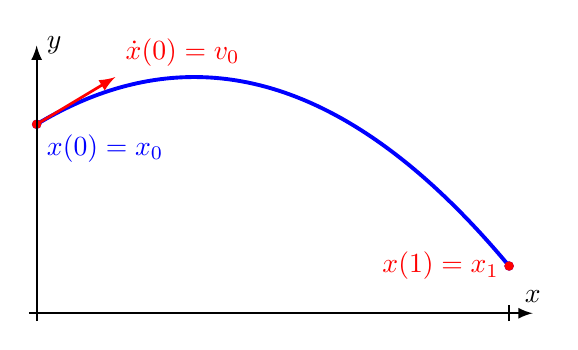
\begin{tikzpicture}[>=latex,thick]

\draw[color=blue,line width=1.4pt]
	plot[domain=0:6,samples=100]
		({\x},{-0.15*(\x-2)*(\x-2)+3});

\xdef\x{0}
\pgfmathparse{-0.15*(\x-2)*(\x-2)+3}
\xdef\y{\pgfmathresult}
\fill[color=blue] (\x,\y) circle[radius=0.06];

\node[color=blue] at (\x,\y) [below right] {$x(0)=x_0$};

\pgfmathparse{0.15*4}
\xdef\m{\pgfmathresult}

\ifthenelse{\boolean{anfang}}{
	\uncover<2->{
		\draw[->,color=red,line width=1pt]
			(\x,\y)--({\x+1.0},{\y+1.0*\m});
		\fill[color=red] (\x,\y) circle[radius=0.06];
		\node[color=red] at ({\x+1},{\y+\m}) [above right]
			{$\dot{x}(0)=v_0$};
	}
}{}

\xdef\x{6}
\pgfmathparse{-0.15*(\x-2)*(\x-2)+3}
\xdef\y{\pgfmathresult}

\ifthenelse{\boolean{anfang}}{
	\fill[color=blue] (\x,\y) circle[radius=0.06];
}{
	\uncover<2->{
		\fill[color=red] (\x,\y) circle[radius=0.06];
		\node[color=red] at (\x,\y) [left] {$x(1)=x_1$};
	}
}

\draw[->] (-0.1,0)--(6.3,0) coordinate[label={$x$}];
\draw[->] (0,-0.1)--(0,3.4) coordinate[label={right:$y$}];
\draw (6,-0.1)--(6,0.1);

\end{tikzpicture}
}

\begin{frame}
\frametitle{Randwertproblem}
\vspace{-15pt}
\begin{columns}[t]
\begin{column}{0.48\hsize}
\begin{block}{Anfangswertproblem}
\vspace{-10pt}
\begin{align*}
\frac{d^2x}{dt^2}
&=
f(t,x,\dot{x})
\\
x(0)&=x_0
\\
{\color<2->{red}\dot{x}(0)}&{\color<2->{red}=v_0}
\end{align*}
\end{block}
\vspace{-25pt}
\begin{center}
\graphik
\end{center}
\end{column}
\begin{column}{0.48\hsize}
\begin{block}{Randwertproblem}
\vspace{-10pt}
\begin{align*}
\frac{d^2x}{dt^2}
&=
f(t,x,\dot{x})
\\
x(0)&=x_0
\\
{\color<2->{red}x(1)}&{\color<2->{red}=x_1}
\end{align*}
\end{block}
\vspace{-25pt}
\begin{center}
\setboolean{anfang}{false}
\graphik
\end{center}
\end{column}
\end{columns}
\end{frame}


\egroup
